\documentclass[11pt,a4paper]{article}
\usepackage[margin=20mm,headheight=16pt]{geometry}
\usepackage{fontspec,kotex,amsmath,booktabs,longtable,array,xcolor,hyperref,fancyhdr,graphicx}
\setmainfont{DejaVu Serif}
\setsansfont{DejaVu Sans}
\setmonofont{DejaVu Sans Mono}
\setmainhangulfont{Noto Sans CJK KR}
\setmonohangulfont{Noto Sans CJK KR}
\definecolor{navy}{HTML}{173E59}
\definecolor{codebg}{HTML}{F3F6F8}
\hypersetup{colorlinks=true,linkcolor=navy,urlcolor=navy,pdftitle={GuardSynth Proposed Method}}
\urlstyle{same}
\setlength{\parindent}{0pt}
\setlength{\parskip}{6pt}
\setlength{\emergencystretch}{4em}
\setlength{\tabcolsep}{4pt}
\renewcommand{\arraystretch}{1.2}
\pagestyle{fancy}\fancyhf{}
\fancyhead[L]{\small GuardSynth}
\fancyhead[R]{\small Proposed Method}
\fancyfoot[C]{\thepage}
\renewcommand{\headrulewidth}{0.3pt}
\clubpenalty=10000\widowpenalty=10000
\raggedbottom
\begin{document}

\section*{IV. Proposed Method}

\section*{A. Overview and Inputs and Outputs}

GuardSynth preserves the action explanation in CoC while making conditions that restrict action selection explicit in a separate specification, then returning those conditions to a natural-language representation. Inputs comprise original CoC, scene observations available for the decision, and applicable rules with their evidence. Outputs comprise structured behavioral constraints, logical verification results under a restricted model, controlled natural language (CNL) generated from the specification, and an augmented learning input. The formal representation specifies condition semantics and verification scope; the language representation conveys those conditions to learning.\par

The process first selects candidate constraints and checks their evidence, then specifies accepted constraints in EBLC. Structural and semantic checks precede conversion to a verification-oriented intermediate representation and SMT queries. CNL corresponding to the specification is subsequently generated and combined with original CoC.\par

\par\medskip\noindent\begin{minipage}{\linewidth}\centering
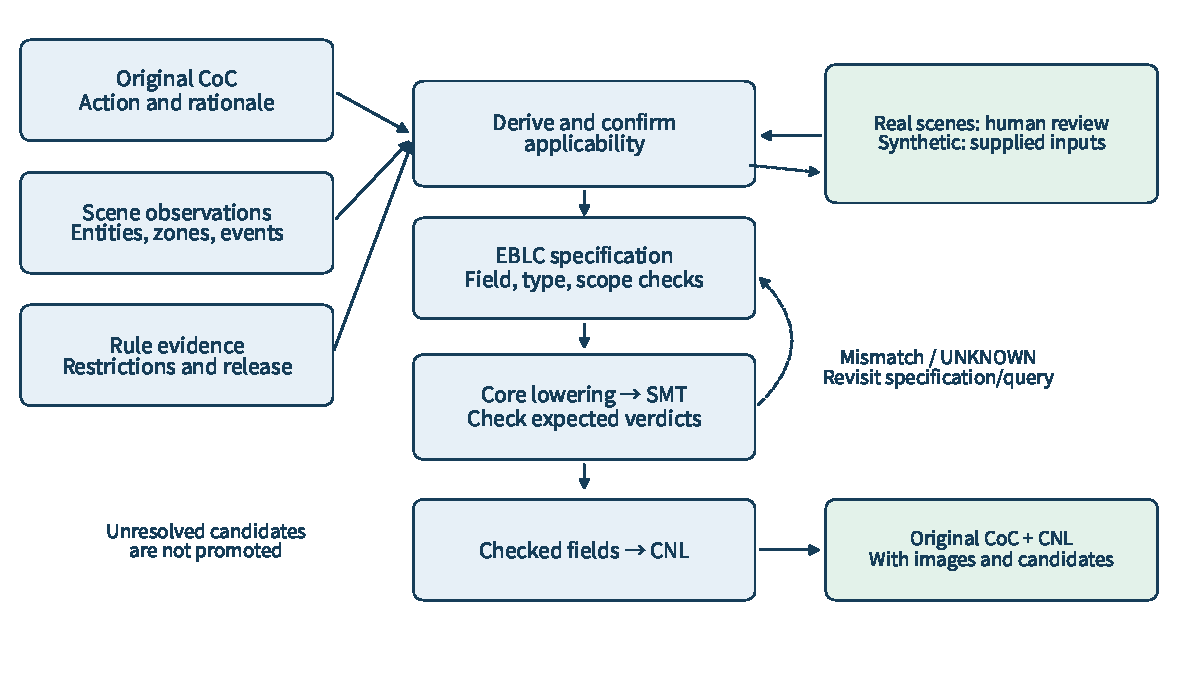
\includegraphics[width=\linewidth,height=.39\textheight,keepaspectratio]{figures/method-flow-en.pdf}
\par\small\raggedright Figure 1. Solid arrows show information flow; dashed arrows return unresolved evidence or unexpected verdicts to the relevant stage. Human confirmation of real scenes is distinguished from supplied synthetic conditions. Structural acceptance alone does not approve scene applicability.
\end{minipage}\par\medskip

Observations, rules, and assumptions have distinct roles. Observations describe entities and events; rules determine restricted actions; assumptions delimit modeled situations. For example, zone clearance time is environmental information, the required subsequent waiting duration is rule information, and the absence of reoccupation is a modeling assumption. Different rules can therefore yield different admissible actions for the same observation.\par

Two executable profiles instantiate this approach. The primary learning experiment constructs numerical temporal contracts from supplied synthetic rules. A separate qualitative profile connects entities, zones, and events through observations and human review of real scenes. Both link specifications to evidence, but their inputs and semantics differ. We use the temporal contract as the running example and the qualitative profile to describe evidence uncertainty and constraint lifecycles. Implementation evidence is linked in \href{\detokenize{../../../../../../projects/04-guardsynth-coc/experiments/paper1_cnl_learning/temporal_preservation.py}}{S1} and \href{\detokenize{../../../../../../platforms/eblc-bcv/src/guard_synth_eblc/action_contract.py}}{S2}.\par

\section*{B. Formal Specification with EBLC}

\subsection*{1. Scope and Elements}

A behavioral constraint restricts available actions in a situation. It differs from an observation, an action rationale, and an objective that ranks admissible actions. Satisfying an entry-permission condition does not force entry; selecting among permitted actions requires a separate objective.\par

Evidence-Bound Lifecycle Contracts (EBLC) represent constraints with their targets, conditions, action restrictions, persistence and release, and evidence. Evidence-Bound denotes explicit links to the inputs on which conditions and rules depend. Lifecycle denotes activation, persistence, release, and, where required, reactivation. This paper uses these organizing principles and implemented restricted profiles, rather than assuming a language covering every traffic situation.\par

\par\medskip\noindent\begin{minipage}{\linewidth}\small
\begin{tabular}{@{}>{\raggedright\arraybackslash}p{\dimexpr 0.2500\linewidth-4.000pt\relax}>{\raggedright\arraybackslash}p{\dimexpr 0.3300\linewidth-5.280pt\relax}>{\raggedright\arraybackslash}p{\dimexpr 0.4200\linewidth-6.720pt\relax}@{}}
\toprule
\textbf{Element} & \textbf{Specification role} & \textbf{Temporal instantiation} \\
\midrule
Subject and target & Whose action is restricted, and with respect to what? & Ego and pedestrian conflict zone \\
Scope & Situation and model of interpretation & Single clearance transition without reoccupation \\
Action restriction & What is disallowed? & Entry before release conditions hold \\
Persistence and release & When does the restriction persist or end? & Required duration following clearance \\
Time and units & Instants, durations, and boundaries & Integer milliseconds; inclusive threshold \\
Evidence and version & Rule sources and interpretation & Rule references and profile version \\
\bottomrule\end{tabular}\end{minipage}\par\medskip

The qualitative profile additionally represents event truth, evidence validity, initial activation, and a policy for combining obligations. These elements address uncertain scene evidence; they are not all evaluated in the primary temporal learning experiment. The proposed modeling scope and experimentally evaluated scope are distinguished.\par

\subsection*{2. Contract Definition and Interpretation}

We use {\ttfamily\small C = (s, z, \ensuremath{\Sigma}, O, E, V)} to explain the two profiles: s denotes the actor, z the target or zone, \ensuremath{\Sigma} the scope and modeling assumptions, O the set of restrictive obligations, E the observation and rule evidence links, and V the interpretation version. This is explanatory notation, not a new six-field JSON schema. Actual serialization follows the restricted profile in Code Box 1.\par

An obligation is interpreted through its activation condition, persistence and release rules, restricted action, and any required initial state. The temporal profile compresses these into a single clearance time and a waiting duration. The qualitative profile updates activation from evidence and the previous state at each decision step. Assumptions and state variables from different profiles are not interchangeable.\par

Let h\_t denote the supplied evidence and state history through decision step t, and a a current action candidate. The meaning of a contract is its admissible candidate set {\ttfamily\small A\_C(h\_t)}. Membership means compatibility with the stated conditions and restrictions. Multiple obligations combine their admissible sets by intersection, requiring all applicable restrictions to hold. The qualitative profile also imposes an entry policy requiring current clearance evidence. Previous inactivity is therefore distinct from current entry permission.\par

An independent objective selects among admissible candidates. Deferral and entry after sufficient waiting may both be permitted while receiving different progress scores. Separating admissibility from optimization prevents interpreting compliance as optimality.\par

\subsection*{3. Temporal Syntax and Semantics}

The temporal profile accepts a structured JSON contract. The following is actual generator output for a 0.5-second waiting rule. Source references provide traceability and contain no target action label.\par

\par\medskip\noindent\begin{minipage}{\linewidth}
\textbf{Code Box 1. Actual generated temporal contract JSON}\par

The input is a supplied 0.5-second waiting rule; the output is a contract containing its target, release condition, and assumptions. Line numbers refer to positions within this box.\par

\par\medskip\noindent\fcolorbox{navy}{codebg}{\begin{minipage}{\dimexpr\linewidth-2\fboxsep-2\fboxrule\relax}
{\small\bfseries Code Box 1}\par\smallskip
\noindent\makebox[1.8em][r]{\color{gray}\scriptsize 1}\hspace{.8em}\parbox[t]{\dimexpr\linewidth-2.8em\relax}{\raggedright\ttfamily\fontsize{8.2}{10.5}\selectfont \hspace*{0.0em}\{\strut}\par\vspace{1pt}
\noindent\makebox[1.8em][r]{\color{gray}\scriptsize 2}\hspace{.8em}\parbox[t]{\dimexpr\linewidth-2.8em\relax}{\raggedright\ttfamily\fontsize{8.2}{10.5}\selectfont \hspace*{1.0em}"version": "supplied-temporal-eblc-profile-v0.1",\strut}\par\vspace{1pt}
\noindent\makebox[1.8em][r]{\color{gray}\scriptsize 3}\hspace{.8em}\parbox[t]{\dimexpr\linewidth-2.8em\relax}{\raggedright\ttfamily\fontsize{8.2}{10.5}\selectfont \hspace*{1.0em}"subject": "ego",\strut}\par\vspace{1pt}
\noindent\makebox[1.8em][r]{\color{gray}\scriptsize 4}\hspace{.8em}\parbox[t]{\dimexpr\linewidth-2.8em\relax}{\raggedright\ttfamily\fontsize{8.2}{10.5}\selectfont \hspace*{1.0em}"target": "pedestrian\_conflict\_zone",\strut}\par\vspace{1pt}
\noindent\makebox[1.8em][r]{\color{gray}\scriptsize 5}\hspace{.8em}\parbox[t]{\dimexpr\linewidth-2.8em\relax}{\raggedright\ttfamily\fontsize{8.2}{10.5}\selectfont \hspace*{1.0em}"hold": "NO\_ENTRY\_WHILE\_OCCUPIED",\strut}\par\vspace{1pt}
\noindent\makebox[1.8em][r]{\color{gray}\scriptsize 6}\hspace{.8em}\parbox[t]{\dimexpr\linewidth-2.8em\relax}{\raggedright\ttfamily\fontsize{8.2}{10.5}\selectfont \hspace*{1.0em}"release\_clear\_ms": 500,\strut}\par\vspace{1pt}
\noindent\makebox[1.8em][r]{\color{gray}\scriptsize 7}\hspace{.8em}\parbox[t]{\dimexpr\linewidth-2.8em\relax}{\raggedright\ttfamily\fontsize{8.2}{10.5}\selectfont \hspace*{1.0em}"time\_unit": "ms",\strut}\par\vspace{1pt}
\noindent\makebox[1.8em][r]{\color{gray}\scriptsize 8}\hspace{.8em}\parbox[t]{\dimexpr\linewidth-2.8em\relax}{\raggedright\ttfamily\fontsize{8.2}{10.5}\selectfont \hspace*{1.0em}"source\_kind": "SUPPLIED\_SYNTHETIC\_RULE",\strut}\par\vspace{1pt}
\noindent\makebox[1.8em][r]{\color{gray}\scriptsize 9}\hspace{.8em}\parbox[t]{\dimexpr\linewidth-2.8em\relax}{\raggedright\ttfamily\fontsize{8.2}{10.5}\selectfont \hspace*{1.0em}"assumption": "SINGLE\_CLEAR\_TRANSITION\_NO\_REOCCUPATION",\strut}\par\vspace{1pt}
\noindent\makebox[1.8em][r]{\color{gray}\scriptsize 10}\hspace{.8em}\parbox[t]{\dimexpr\linewidth-2.8em\relax}{\raggedright\ttfamily\fontsize{8.2}{10.5}\selectfont \hspace*{1.0em}"source\_refs": [\strut}\par\vspace{1pt}
\noindent\makebox[1.8em][r]{\color{gray}\scriptsize 11}\hspace{.8em}\parbox[t]{\dimexpr\linewidth-2.8em\relax}{\raggedright\ttfamily\fontsize{8.2}{10.5}\selectfont \hspace*{2.0em}"Project01/temporal\_guard\_world.py::\_guard",\strut}\par\vspace{1pt}
\noindent\makebox[1.8em][r]{\color{gray}\scriptsize 12}\hspace{.8em}\parbox[t]{\dimexpr\linewidth-2.8em\relax}{\raggedright\ttfamily\fontsize{8.2}{10.5}\selectfont \hspace*{2.0em}"paper1-method-preservation-v0.1"\strut}\par\vspace{1pt}
\noindent\makebox[1.8em][r]{\color{gray}\scriptsize 13}\hspace{.8em}\parbox[t]{\dimexpr\linewidth-2.8em\relax}{\raggedright\ttfamily\fontsize{8.2}{10.5}\selectfont \hspace*{1.0em}]\strut}\par\vspace{1pt}
\noindent\makebox[1.8em][r]{\color{gray}\scriptsize 14}\hspace{.8em}\parbox[t]{\dimexpr\linewidth-2.8em\relax}{\raggedright\ttfamily\fontsize{8.2}{10.5}\selectfont \hspace*{0.0em}\}\strut}\par\vspace{1pt}
\end{minipage}}\par\medskip
\end{minipage}\par\medskip

The {\ttfamily\small subject} and {\ttfamily\small target} identify the actor and restricted zone. The {\ttfamily\small hold} field specifies no entry during occupancy; {\ttfamily\small release\_clear\_ms} specifies waiting after clearance. The {\ttfamily\small assumption} field specifies one occupied-to-clear transition without subsequent reoccupation. This permits continuous clearance to be represented by one clearance time and an elapsed duration.\par

In Code Box 1, lines 2–5 fix the version and restriction target; lines 6–7 specify duration and units. Lines 8–9 identify the supplied synthetic rule and no-reoccupation assumption, while lines 10–13 preserve source references. Environmental clearance and candidate entry times are bound separately rather than mixed into this rule JSON.\par

Evaluation separately binds environmental clearance time {\ttfamily\small clear\_ms}, candidate entry time {\ttfamily\small entry\_ms}, and Boolean entry indicator {\ttfamily\small enters}. Both times use integer milliseconds. The restriction is:\par

\[\mathit{enters}\ \Longrightarrow\ \mathit{entry\_ms}\geq\mathit{clear\_ms}+\mathit{release\_clear\_ms}.\]

For {\ttfamily\small clear\_ms = 11000} and {\ttfamily\small release\_clear\_ms = 500}, an entering candidate is compatible only at or after 11500ms. The inclusive comparison admits 11500ms but excludes 11499ms. A non-entering candidate has {\ttfamily\small enters = false} and does not violate this entry restriction; its progress is assessed separately.\par

The validator checks the supported version and fixed field combinations. Supported durations are 500, 1500, 800, and 1800ms; the primary expanded learning dataset uses 500 and 1500ms. The implementation accepts a restricted profile with defined interpretation, not arbitrary JSON as a general contract. \href{\detokenize{../../../../../../projects/04-guardsynth-coc/experiments/paper1_cnl_learning/temporal_preservation.py}}{S1}, \href{\detokenize{../../../../../../projects/04-guardsynth-coc/experiments/paper1_cnl_learning/temporal_training_data.py}}{S3}\par

Writing {\ttfamily\small \ensuremath{\tau} = clear\_ms}, {\ttfamily\small \ensuremath{\Delta} = release\_clear\_ms}, {\ttfamily\small u = entry\_ms}, and {\ttfamily\small e = enters} gives {\ttfamily\small P\_C(e,u,\ensuremath{\tau}) = (\ensuremath{\neg}e) \ensuremath{\lor} (u \ensuremath{\geq} \ensuremath{\tau} + \ensuremath{\Delta})}. Candidates satisfying P\_C belong to the temporal admissible set. Entry requires elapsed time {\ttfamily\small u \ensuremath{-} \ensuremath{\tau} \ensuremath{\geq} \ensuremath{\Delta}}; non-entry satisfies the restriction independently of its entry-time variable. Both \ensuremath{\tau} and u are instants, whereas \ensuremath{\Delta} is a duration. This distinguishes a zone being clear from having remained clear for the required duration.\par

\subsection*{4. Qualitative Lifecycle Semantics}

The real-scene profile uses {\ttfamily\small truth[j,t]}, {\ttfamily\small valid[j,t]}, and {\ttfamily\small active[j,t]} for obligation j at decision step t. Truth values are TRUE, FALSE, UNKNOWN, and CONFLICT. FALSE denotes confirmed resolution of the restricting condition, not mere absence of an observation. Validity denotes admissibility of the evidence. Activation records whether the obligation is active; its value before the first decision is a separate input.\par

\par\medskip\noindent\begin{minipage}{\linewidth}
\textbf{Code Box 2. Pseudocode for evidence-based state updates}\par

Inputs are the current truth value and evidence validity for obligation j, together with previous activation; the output is current activation. This is explanatory pseudocode, not a verbatim source excerpt.\par

\par\medskip\noindent\fcolorbox{navy}{codebg}{\begin{minipage}{\dimexpr\linewidth-2\fboxsep-2\fboxrule\relax}
{\small\bfseries Code Box 2}\par\smallskip
\noindent\makebox[1.8em][r]{\color{gray}\scriptsize 1}\hspace{.8em}\parbox[t]{\dimexpr\linewidth-2.8em\relax}{\raggedright\ttfamily\fontsize{8.2}{10.5}\selectfont \hspace*{0.0em}on[j,t] = valid[j,t] AND (truth[j,t] = TRUE)\strut}\par\vspace{1pt}
\noindent\makebox[1.8em][r]{\color{gray}\scriptsize 2}\hspace{.8em}\parbox[t]{\dimexpr\linewidth-2.8em\relax}{\raggedright\ttfamily\fontsize{8.2}{10.5}\selectfont \hspace*{0.0em}clear[j,t] = valid[j,t] AND (truth[j,t] = FALSE)\strut}\par\vspace{1pt}
\noindent\makebox[1.8em][r]{\color{gray}\scriptsize 3}\hspace{.8em}\parbox[t]{\dimexpr\linewidth-2.8em\relax}{\raggedright\ttfamily\fontsize{8.2}{10.5}\selectfont \hspace*{0.0em}active[j,t] = TRUE,             if on[j,t]\strut}\par\vspace{1pt}
\noindent\makebox[1.8em][r]{\color{gray}\scriptsize 4}\hspace{.8em}\parbox[t]{\dimexpr\linewidth-2.8em\relax}{\raggedright\ttfamily\fontsize{8.2}{10.5}\selectfont \hspace*{7.0em}FALSE,           else if clear[j,t]\strut}\par\vspace{1pt}
\noindent\makebox[1.8em][r]{\color{gray}\scriptsize 5}\hspace{.8em}\parbox[t]{\dimexpr\linewidth-2.8em\relax}{\raggedright\ttfamily\fontsize{8.2}{10.5}\selectfont \hspace*{7.0em}previous\_active, otherwise\strut}\par\vspace{1pt}
\end{minipage}}\par\medskip
\end{minipage}\par\medskip

Evidence is read and activation updated before constraining the action. Valid activation evidence activates an obligation, valid clearance evidence releases it, and otherwise its previous state persists. The same rule reactivates it when the activation condition is confirmed again. Explicit ordering and initialization fix the interpretation at each step.\par

The current policy permits entry only when clearance of every declared obligation is confirmed. Previous inactivity alone does not permit entry if current clearance is unconfirmed. When all obligations are clear, both entry and deferral are allowed. Permission is not a liveness guarantee requiring progress. UNKNOWN and CONFLICT are evidence states, distinct from an SMT solver returning UNKNOWN when it cannot decide a query. \href{\detokenize{../../../../../../platforms/eblc-bcv/src/guard_synth_eblc/action_contract.py}}{S2}\par

Lines 1–2 of Code Box 2 require both validity and the corresponding truth value. Lines 3–5 select activation, release, or persistence. At the first step, {\ttfamily\small previous\_active} is the explicit {\ttfamily\small prior\_active} input; subsequently it is activation at the preceding step. A single truth value cannot be both TRUE and FALSE, so activation and clearance cannot simultaneously hold in this encoding.\par

\par\medskip\noindent\begin{minipage}{\linewidth}\centering
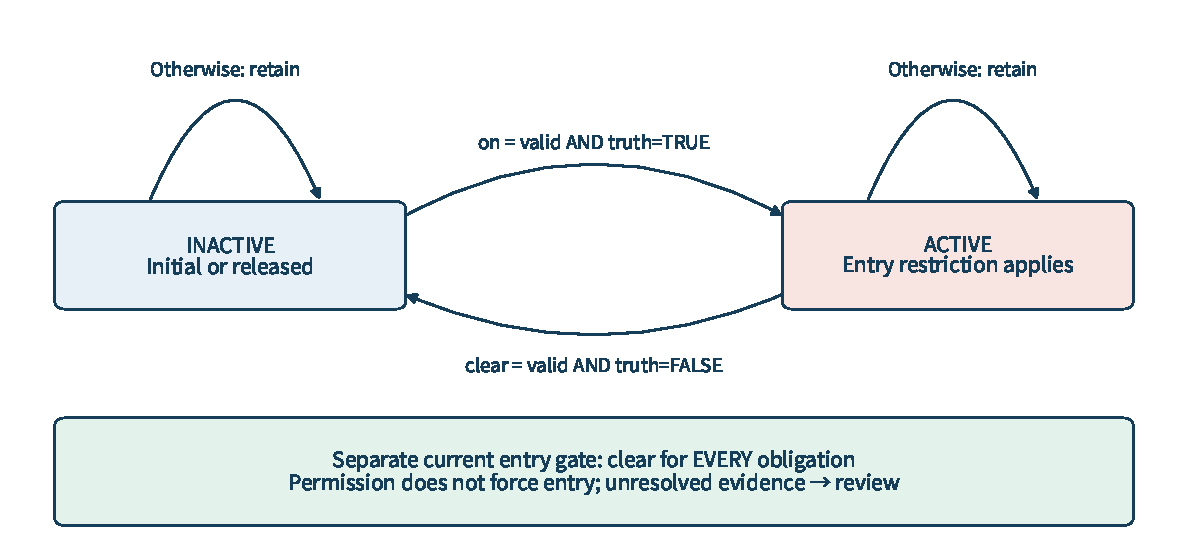
\includegraphics[width=\linewidth,height=.39\textheight,keepaspectratio]{figures/lifecycle-en.pdf}
\par\small\raggedright Figure 2. The upper panel shows one obligation's transitions; the lower panel combines all obligations for current entry permission. Inactivity includes both release and initial inactivity. There is no edge equating inactivity alone with entry permission.
\end{minipage}\par\medskip

The policy is {\ttfamily\small entry\_permitted[t] = AND\_j clear[j,t]}; ENTER\_ZONE requires this value to be true. DEFER\_ENTRY does not violate this entry restriction. Unknown, conflicting, or invalid evidence separately sets {\ttfamily\small review\_required}. For example, starting from inactivity, valid evidence TRUE \ensuremath{\rightarrow} UNKNOWN \ensuremath{\rightarrow} FALSE \ensuremath{\rightarrow} TRUE yields active \ensuremath{\rightarrow} active \ensuremath{\rightarrow} inactive \ensuremath{\rightarrow} active. Entry is permitted only at the third decision, where deferral remains possible. This is a constructed semantic illustration.\par

\section*{C. Defining and Deriving Behavioral Constraints}

\subsection*{1. Separating Candidate Constraints from Evidence}

Not every CoC sentence becomes a constraint. “A pedestrian is crossing” is an observational claim; “yield to protect the pedestrian” is an action rationale. “Do not enter while the zone is occupied” contains a condition and restriction, making it a constraint candidate. “Choose the admissible candidate with greatest progress” is a selection objective. This distinction avoids inventing thresholds or release conditions absent from the explanation and its evidence.\par

Inputs serve three evidence roles. CoC identifies potentially relevant actions and obligations. Scene observations bind entities, zones, events, and times. Supplied rules or separately established normative evidence determine applicability and restriction content. A sentence appearing in CoC does not itself confirm applicability to the current scene.\par

\subsection*{2. Specification Procedure and Automation Scope}

The procedure identifies action-relevant entities, situations, and rationales in CoC, then binds entities and zones to observations and identifies the decision time. Rule evidence determines the restricted action and applicability conditions; persistence, release, timing, and assumptions are subsequently specified. Unconfirmed information remains unresolved rather than becoming an observed fact. Accepted content is mapped to supported fields with evidence references and version information.\par

In the primary synthetic experiment, the environment generator and supplied rule provide these inputs. Environmental clearance and rule duration determine the contract and verification representation. Automation structures and transforms given conditions; it does not discover traffic law or waiting durations from video alone. The real-scene path involves human confirmation of entities, zones, events, and applicability, and the implemented adapter is limited to a particular review task. \href{\detokenize{../../../../../../projects/04-guardsynth-coc/experiments/paper1_cnl_learning/temporal_training_data.py}}{S3}, \href{\detokenize{../../../../../../projects/04-guardsynth-coc/src/guard_synth/qualitative_scene_contract.py}}{S4}\par

Constraints and learning references are managed separately. Defining admissibility does not automatically establish a real-scene ground-truth action. For the synthetic task, separate integer arithmetic uses known environmental states and rules to identify admissible candidates, then selects the one with greatest progress. This calculation does not copy its answer from CNL or an SMT verdict, but shares the environmental and rule assumptions.\par

\par\medskip\noindent\begin{minipage}{\linewidth}\centering
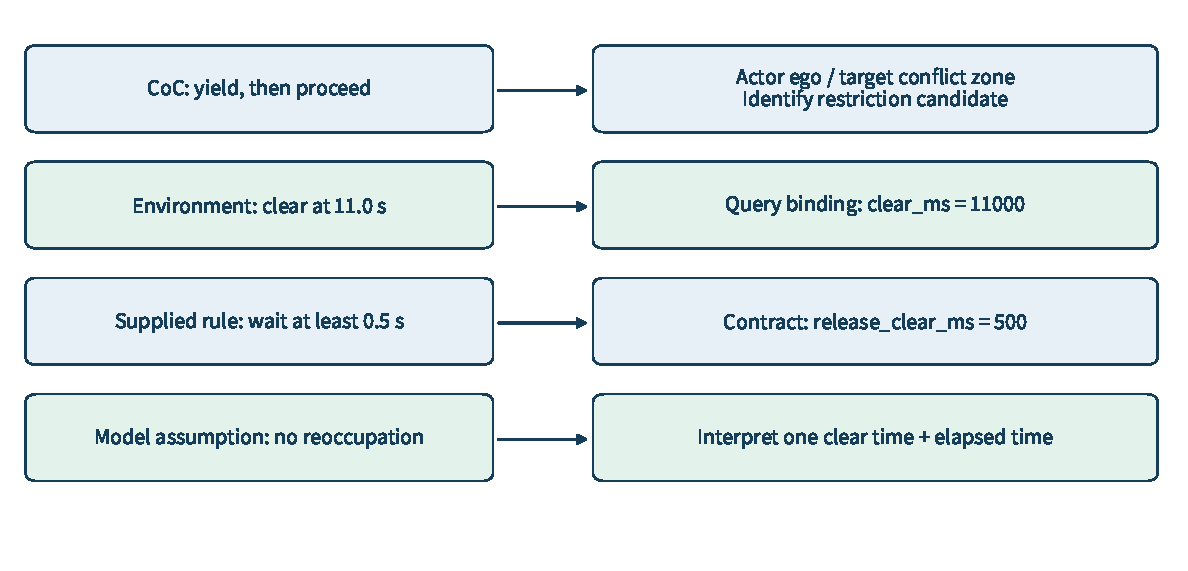
\includegraphics[width=\linewidth,height=.39\textheight,keepaspectratio]{figures/evidence-map-en.pdf}
\par\small\raggedright Figure 3. Environmental clearance at 11.0 seconds binds a query variable, whereas the supplied 0.5-second duration becomes a contract field. No reoccupation is an assumption needed to connect these values through a temporal inequality. Derivation distinguishes these roles when constructing evidence-supported fields.
\end{minipage}\par\medskip

\subsection*{3. Running Temporal Example}

Original CoC reads “Yield to the crossing pedestrian, then proceed through the intersection.” The environment supplies clearance at 11.0 seconds; a separate rule requires a minimum wait of 0.5 or 1.5 seconds. The duration is an explicit experimental condition, not a value inferred from CoC or a universal traffic-law requirement.\par

\par\medskip\noindent\begin{minipage}{\linewidth}\small
\begin{tabular}{@{}>{\raggedright\arraybackslash}p{\dimexpr 0.1500\linewidth-4.800pt\relax}>{\raggedright\arraybackslash}p{\dimexpr 0.1800\linewidth-5.760pt\relax}>{\raggedright\arraybackslash}p{\dimexpr 0.1900\linewidth-6.080pt\relax}>{\raggedright\arraybackslash}p{\dimexpr 0.2400\linewidth-7.680pt\relax}>{\raggedright\arraybackslash}p{\dimexpr 0.2400\linewidth-7.680pt\relax}@{}}
\toprule
\textbf{Candidate} & \textbf{Entry time} & \textbf{Progress score} & \textbf{0.5-second wait} & \textbf{1.5-second wait} \\
\midrule
A & 10.5s & 110 & Violates & Violates \\
B & 11.5s & 100 & Admissible; reference & Violates \\
C & 12.5s & 85 & Admissible & Admissible; reference \\
D & No entry & 0 & Admissible & Admissible \\
\bottomrule\end{tabular}\end{minipage}\par\medskip

Progress is a synthetic utility, not measured distance or speed. B maximizes admissible progress under the 0.5-second contract and C under the 1.5-second contract. D violates neither but does not complete the progress objective. The table is a generated data instance, not evidence of actual model predictions. Candidate labels rotate during dataset construction to avoid linking the answer to a fixed letter.\par

\section*{D. Verifying EBLC Specifications Linked to CoC}

\subsection*{1. Binding Checks and Core Lowering}

Verification requires semantic input binding and logical queries. Subject, zone, event time, and duration must refer to the same case, and specifications must satisfy supported version, field, and unit requirements. Evidence identifiers support traceability rather than proving factual truth. Unbound fields are distinguished from completed scene bindings; passing syntax checks does not turn a conditional specification into reviewed learning data.\par

Temporal contracts lower to Core declarations of Boolean {\ttfamily\small enters} and integer {\ttfamily\small clear\_ms} and {\ttfamily\small entry\_ms}; {\ttfamily\small release\_clear\_ms} becomes an integer constant. Core is an intermediate representation of declarations and logical clauses, type-checked before SMT compilation. Time uses integer millisecond ticks with Core unit marker {\ttfamily\small 1}, not seconds. Variables in this profile are time-invariant and the clause is enforced initially. The configured {\ttfamily\small horizon = 2} is a model bound, not verification of a two-second driving trajectory. \href{\detokenize{../../../../../../projects/04-guardsynth-coc/experiments/paper1_cnl_learning/temporal_preservation.py}}{S1}\par

\subsection*{2. Properties and Queries}

\par\medskip\noindent\begin{minipage}{\linewidth}\centering
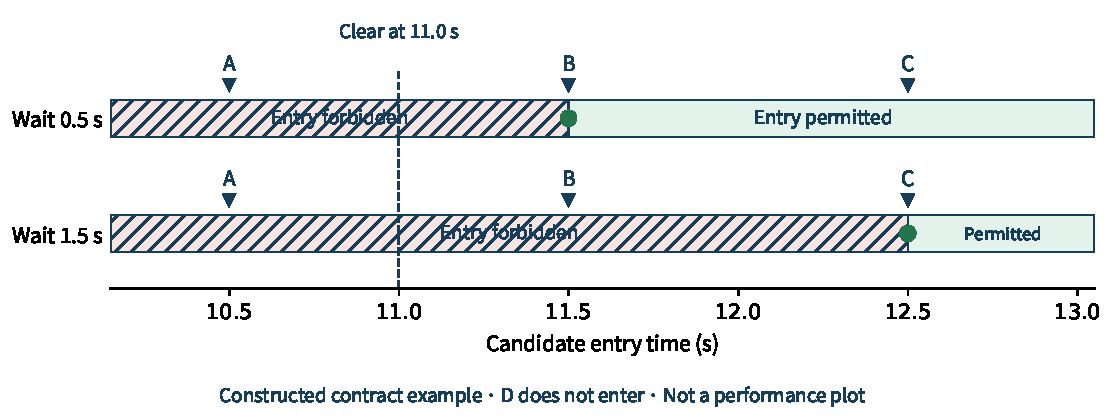
\includegraphics[width=\linewidth,height=.39\textheight,keepaspectratio]{figures/temporal-boundary-en.pdf}
\par\small\raggedright Figure 4. The horizontal axis is entry time in seconds. The same clearance event yields admissibility from 11.5 or 12.5 seconds depending on the duration. Closed boundary points include the threshold instant. D is a non-entry candidate, not a point on this axis. The graph computes contract semantics rather than model accuracy or measured driving performance.
\end{minipage}\par\medskip

We distinguish consistency, restriction enforcement, release boundaries, and permissibility. Base SAT establishes a satisfying model, but non-entry alone can satisfy the specification. We therefore separately check that an entering model exists after release. This avoids specifications that exclude all entry without substituting for measurement of actual model progress.\par

\par\medskip\noindent\begin{minipage}{\linewidth}\small
\begin{tabular}{@{}>{\raggedright\arraybackslash}p{\dimexpr 0.2200\linewidth-5.280pt\relax}>{\raggedright\arraybackslash}p{\dimexpr 0.2000\linewidth-4.800pt\relax}>{\raggedright\arraybackslash}p{\dimexpr 0.3000\linewidth-7.200pt\relax}>{\raggedright\arraybackslash}p{\dimexpr 0.2800\linewidth-6.720pt\relax}@{}}
\toprule
\textbf{Property} & \textbf{Query} & \textbf{Expected} & \textbf{Interpretation} \\
\midrule
Consistency & Base contract & SAT & A satisfying case exists \\
Restriction & Entry earlier than release & UNSAT & Early entry and contract are incompatible \\
Before boundary & Entry at 11.499s; wait 0.5s & UNSAT & Entry just before release is excluded \\
At boundary & Entry at 11.500s; wait 0.5s & SAT & Equality is permitted \\
After boundary & Entry at 11.501s; wait 0.5s & SAT & Entry after release is feasible \\
Deferral & enters is false & SAT & Entry is not forced \\
\bottomrule\end{tabular}\end{minipage}\par\medskip

Concrete times assume clearance at 11.0 seconds. The restriction query searches for a counterexample with {\ttfamily\small enters} true and {\ttfamily\small entry\_ms < clear\_ms + release\_clear\_ms}. This is symbolic rather than fixing both time variables; boundary rows bind concrete values. Even the symbolic result concerns the encoded inequality and assumptions, not video interpretation or rule selection.\par

The six manuscript queries were executed for both 500ms and 1500ms contracts, yielding 12 matching verdicts. The existing bridge's 100 queries were rerun separately. Neither set constitutes new learning-effect evidence. Records preserve each query, expected and observed verdicts, and actual SMT-LIB output. \href{\detokenize{../methodology-2026-09-30-001/manuscript_examples.json}}{S5}\par

\subsection*{3. SMT Representation and Interpretation}

The following readable SMT-LIB example expresses the core 0.5-second restriction. It is an explanatory representation, not the entire compiler output, which is retained in separate query files.\par

\par\medskip\noindent\begin{minipage}{\linewidth}
\textbf{Code Box 3. Executable SMT-LIB example comparing early and boundary entry}\par

Inputs are the contract duration and clearance at 11000ms. Each candidate time is fixed in turn to query compatibility with the contract.\par

\par\medskip\noindent\fcolorbox{navy}{codebg}{\begin{minipage}{\dimexpr\linewidth-2\fboxsep-2\fboxrule\relax}
{\small\bfseries Code Box 3}\par\smallskip
\noindent\makebox[1.8em][r]{\color{gray}\scriptsize 1}\hspace{.8em}\parbox[t]{\dimexpr\linewidth-2.8em\relax}{\raggedright\ttfamily\fontsize{8.2}{10.5}\selectfont \hspace*{0.0em}(declare-const enters Bool)\strut}\par\vspace{1pt}
\noindent\makebox[1.8em][r]{\color{gray}\scriptsize 2}\hspace{.8em}\parbox[t]{\dimexpr\linewidth-2.8em\relax}{\raggedright\ttfamily\fontsize{8.2}{10.5}\selectfont \hspace*{0.0em}(declare-const entry\_ms Int)\strut}\par\vspace{1pt}
\noindent\makebox[1.8em][r]{\color{gray}\scriptsize 3}\hspace{.8em}\parbox[t]{\dimexpr\linewidth-2.8em\relax}{\raggedright\ttfamily\fontsize{8.2}{10.5}\selectfont \hspace*{0.0em}(declare-const clear\_ms Int)\strut}\par\vspace{1pt}
\noindent\makebox[1.8em][r]{\color{gray}\scriptsize 4}\hspace{.8em}\parbox[t]{\dimexpr\linewidth-2.8em\relax}{\raggedright\ttfamily\fontsize{8.2}{10.5}\selectfont \hspace*{0.0em}(assert (= clear\_ms 11000))\strut}\par\vspace{1pt}
\noindent\makebox[1.8em][r]{\color{gray}\scriptsize 5}\hspace{.8em}\parbox[t]{\dimexpr\linewidth-2.8em\relax}{\raggedright\ttfamily\fontsize{8.2}{10.5}\selectfont \hspace*{0.0em}(assert (=> enters (>= entry\_ms (+ clear\_ms 500))))\strut}\par\vspace{1pt}
\noindent\makebox[1.8em][r]{\color{gray}\scriptsize 6}\hspace{.8em}\parbox[t]{\dimexpr\linewidth-2.8em\relax}{\raggedright\ttfamily\fontsize{8.2}{10.5}\selectfont \hspace*{0.0em}(assert enters)\strut}\par\vspace{1pt}
\noindent\makebox[1.8em][r]{\color{gray}\scriptsize 7}\hspace{.8em}\parbox[t]{\dimexpr\linewidth-2.8em\relax}{\raggedright\ttfamily\fontsize{8.2}{10.5}\selectfont \hspace*{0.0em}(push)\strut}\par\vspace{1pt}
\noindent\makebox[1.8em][r]{\color{gray}\scriptsize 8}\hspace{.8em}\parbox[t]{\dimexpr\linewidth-2.8em\relax}{\raggedright\ttfamily\fontsize{8.2}{10.5}\selectfont \hspace*{0.0em}(assert (= entry\_ms 11499))\strut}\par\vspace{1pt}
\noindent\makebox[1.8em][r]{\color{gray}\scriptsize 9}\hspace{.8em}\parbox[t]{\dimexpr\linewidth-2.8em\relax}{\raggedright\ttfamily\fontsize{8.2}{10.5}\selectfont \hspace*{0.0em}(check-sat) ; unsat\strut}\par\vspace{1pt}
\noindent\makebox[1.8em][r]{\color{gray}\scriptsize 10}\hspace{.8em}\parbox[t]{\dimexpr\linewidth-2.8em\relax}{\raggedright\ttfamily\fontsize{8.2}{10.5}\selectfont \hspace*{0.0em}(pop)\strut}\par\vspace{1pt}
\noindent\makebox[1.8em][r]{\color{gray}\scriptsize 11}\hspace{.8em}\parbox[t]{\dimexpr\linewidth-2.8em\relax}{\raggedright\ttfamily\fontsize{8.2}{10.5}\selectfont \hspace*{0.0em}(push)\strut}\par\vspace{1pt}
\noindent\makebox[1.8em][r]{\color{gray}\scriptsize 12}\hspace{.8em}\parbox[t]{\dimexpr\linewidth-2.8em\relax}{\raggedright\ttfamily\fontsize{8.2}{10.5}\selectfont \hspace*{0.0em}(assert (= entry\_ms 11500))\strut}\par\vspace{1pt}
\noindent\makebox[1.8em][r]{\color{gray}\scriptsize 13}\hspace{.8em}\parbox[t]{\dimexpr\linewidth-2.8em\relax}{\raggedright\ttfamily\fontsize{8.2}{10.5}\selectfont \hspace*{0.0em}(check-sat) ; sat\strut}\par\vspace{1pt}
\noindent\makebox[1.8em][r]{\color{gray}\scriptsize 14}\hspace{.8em}\parbox[t]{\dimexpr\linewidth-2.8em\relax}{\raggedright\ttfamily\fontsize{8.2}{10.5}\selectfont \hspace*{0.0em}(pop)\strut}\par\vspace{1pt}
\end{minipage}}\par\medskip
\end{minipage}\par\medskip

The first UNSAT verdict indicates incompatibility of early entry with the specification, not a defective specification. The second SAT verdict indicates compatibility of the selected entry. Neither includes optimality or real-world safety. UNKNOWN or unexpected verdicts are not accepted as successful verification. Structural checks, scene binding, logical verification, and CNL correspondence serve different roles.\par

Lines 1–3 of Code Box 3 declare types; line 4 binds environmental clearance and line 5 states the restriction. Line 6 excludes satisfying the query through non-entry. Lines 7–10 temporarily add 11499ms, obtain UNSAT, and remove that candidate condition. Lines 11–14 add 11500ms to the same base contract and obtain SAT. The push/pop scopes prevent both candidate conditions from remaining simultaneously and causing an artificial contradiction.\par

\section*{E. CNL Generation and CoC Augmentation}

\subsection*{1. Generating Sentences from Verified Specifications}

CNL is generated from checked fields through fixed sentence rules. The temporal renderer accepts structurally validated contracts and maps zone and duration to text. It does not itself invoke the solver; specification verification precedes rendering. Candidate labels, reference actions, and progress scores are not generator arguments. \href{\detokenize{../../../../../../projects/04-guardsynth-coc/experiments/paper1_cnl_learning/temporal_preservation.py}}{S1}\par

\par\medskip\noindent\begin{minipage}{\linewidth}
\textbf{Code Box 4. Verbatim excerpt of the CNL generator}\par

The following is the actual render function in S1. Input raw is a temporal contract; the return value contains two sentences. Numbers count logical source lines; long lines wrap within the box.\par

\par\medskip\noindent\fcolorbox{navy}{codebg}{\begin{minipage}{\dimexpr\linewidth-2\fboxsep-2\fboxrule\relax}
{\small\bfseries Code Box 4}\par\smallskip
\noindent\makebox[1.8em][r]{\color{gray}\scriptsize 1}\hspace{.8em}\parbox[t]{\dimexpr\linewidth-2.8em\relax}{\raggedright\ttfamily\fontsize{8.2}{10.5}\selectfont \hspace*{0.0em}def render(raw):\strut}\par\vspace{1pt}
\noindent\makebox[1.8em][r]{\color{gray}\scriptsize 2}\hspace{.8em}\parbox[t]{\dimexpr\linewidth-2.8em\relax}{\raggedright\ttfamily\fontsize{8.2}{10.5}\selectfont \hspace*{2.0em}validate(raw)\strut}\par\vspace{1pt}
\noindent\makebox[1.8em][r]{\color{gray}\scriptsize 3}\hspace{.8em}\parbox[t]{\dimexpr\linewidth-2.8em\relax}{\raggedright\ttfamily\fontsize{8.2}{10.5}\selectfont \hspace*{2.0em}\# Render only validated contract fields, never scene target/candidate/answer.\strut}\par\vspace{1pt}
\noindent\makebox[1.8em][r]{\color{gray}\scriptsize 4}\hspace{.8em}\parbox[t]{\dimexpr\linewidth-2.8em\relax}{\raggedright\ttfamily\fontsize{8.2}{10.5}\selectfont \hspace*{2.0em}return ('Do not enter the pedestrian conflict zone while it is occupied. '\strut}\par\vspace{1pt}
\noindent\makebox[1.8em][r]{\color{gray}\scriptsize 5}\hspace{.8em}\parbox[t]{\dimexpr\linewidth-2.8em\relax}{\raggedright\ttfamily\fontsize{8.2}{10.5}\selectfont \hspace*{6.0em}f'Enter only after the zone has remained clear for at least \{raw["release\_clear\_ms"]/1000:.1f\} s.')\strut}\par\vspace{1pt}
\end{minipage}}\par\medskip
\end{minipage}\par\medskip

Line 2 requires an exact match to a supported contract. Since validation also fixes the target and restriction type, line 4 can emit a constant zone phrase. Line 5 converts milliseconds to seconds with one decimal place, exactly representing the currently supported durations. The function neither invokes the solver nor selects a target action. Other targets or arbitrary precision would require a separate extension.\par

Actual output for the 0.5-second contract is:\par

\begin{quote}Do not enter the pedestrian conflict zone while it is occupied. Enter only after the zone has remained clear for at least 0.5 s.\end{quote}

The first sentence identifies the zone and occupancy restriction; the second expresses release and duration. “At least” corresponds to an inclusive boundary, and “only after” specifies a necessary condition rather than an instruction to enter. The conversion maps 500ms to 0.5s and, under the same rule, 1500ms to 1.5s. Correspondence is interpreted for supported durations and the single-clearance, no-reoccupation assumption.\par

\par\medskip\noindent\begin{minipage}{\linewidth}\centering
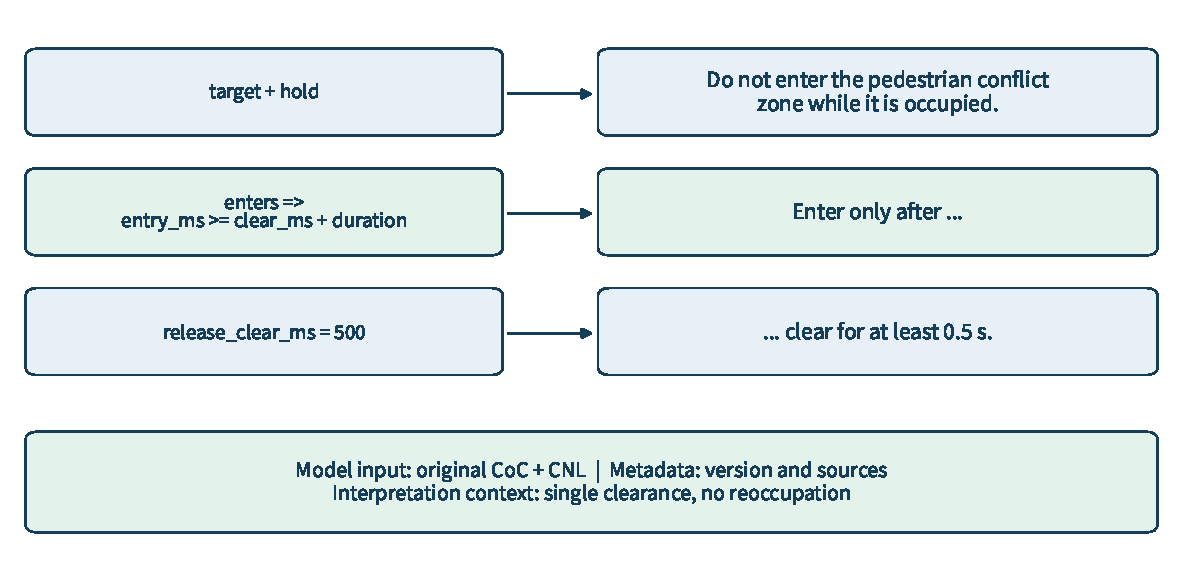
\includegraphics[width=\linewidth,height=.39\textheight,keepaspectratio]{figures/cnl-map-en.pdf}
\par\small\raggedright Figure 5. Target and restriction map to the first sentence; release duration and the inclusive boundary map to the second. Original CoC and CNL enter the model together, while source and version metadata remain separately traceable. Colors distinguish mappings, not additional levels of verification.
\end{minipage}\par\medskip

\subsection*{2. Scope of Semantic Correspondence}

Generation preserves target, negation, conditional direction, value, and unit. Omitting “at least” or replacing “enter only after” with a requirement to enter after clearance would change admissibility. Fixed field mappings make these relationships explicit and inspectable.\par

Not all metadata appears in model-facing sentences. Versions and source references remain traceability metadata; CNL conveys action-relevant conditions. Modeling assumptions are specified in the environment and task definition. The claim is correspondence of action restrictions within that context, not literal one-to-one rendering of every JSON field. Freely rewritten sentences or additional profiles require separate semantic review.\par

\subsection*{3. Combining CNL with Learning Inputs}

Original CoC provides an action rationale, and CNL supplies additional behavioral conditions. They are combined without replacing CoC with a specification. The augmented example reads:\par

\begin{quote}Yield to the crossing pedestrian, then proceed through the intersection. Do not enter the pedestrian conflict zone while it is occupied. Enter only after the zone has remained clear for at least 0.5 s.\end{quote}

The image and action candidates accompany this text, while a separate reference calculation supplies the target label. P0 receives original CoC, P1 receives CoC with the existing natural-language constraint, and P2 receives CoC with EBLC-derived CNL. P1 and P2 both add constraints; their primary comparator is CoC-only P0. Raw EBLC JSON and solver verdicts are not supplied as answer hints.\par

P1 and P2 receive constraints during both training and evaluation. This evaluates selection using explicit rules, not directly whether identical behavior persists without evaluation-time constraints. P0 lacks the waiting duration, so its inputs can be identical for paired contracts requiring different reference actions. This information difference is disclosed as part of the comparison.\par

Traceable records retain image references, CoC, contracts and evidence, CNL, candidates, reference actions, and splits, separating model-visible fields from answers and verification fields. This supports reconstruction of what was specified from which evidence, how it was expressed, and which action served as the learning target. Training budgets and metrics are presented in the experimental section.\par

\begingroup\small\setlength{\parskip}{3pt}
\subsection*{Implementation and Example Evidence}

These links provide reproducibility evidence for manuscript review, separate from external related-work citations. They will connect to code and data availability and supplementary material in the integrated manuscript.\par

\begin{itemize}\setlength{\itemsep}{0pt}\setlength{\parsep}{0pt}\setlength{\topsep}{2pt}
\item \href{\detokenize{../../../../../../projects/04-guardsynth-coc/experiments/paper1_cnl_learning/temporal_preservation.py}}{S1 Temporal contracts, Core lowering, verification, and CNL generation}
\item \href{\detokenize{../../../../../../platforms/eblc-bcv/src/guard_synth_eblc/action_contract.py}}{S2 Qualitative contract parsing and lifecycle semantics}
\item \href{\detokenize{../../../../../../projects/04-guardsynth-coc/experiments/paper1_cnl_learning/temporal_training_data.py}}{S3 Learning inputs and independent reference calculation}
\item \href{\detokenize{../../../../../../projects/04-guardsynth-coc/src/guard_synth/qualitative_scene_contract.py}}{S4 Restricted real-scene adapter}
\item \href{\detokenize{../methodology-2026-09-30-001/manuscript_examples.json}}{S5 Executed manuscript queries and results}
\item \href{\detokenize{../methodology-2026-09-30-001/learning_input_examples.json}}{Two example learning-input records}
\end{itemize}
\endgroup
\end{document}